%%%%%%%%%%%%%%%%%%%%%%%%%%%%%%%%%%%%%%%%%%%%%%%%%%%%%%%%%%%%%%%%%%%%%%%%%%%%%
%集録提出用のサンプルファイルです。
%このファイルを参考にして集録を作成してください。
%%%%%%%%%%%%%%%%%%%%%%%%%%%%%%%%%%%%%%%%%%%%%%%%%%%%%%%%%%%%%%%%%%%%%%%%%%%%%
%%%%%%%%%%%%%%%%%%%%%%%%%%%%%%%%%%%%%%%%%%%%%%%%%%%%%%%%%%%%%%%%%%%%%%%%%%%%%
\documentclass[a4paper,10pt,oneside,twocolumn,notitlepage,final]{jarticle}
\usepackage{ss17(UTF-8)}
%%%%%%%%%%%%%%%%%%%%%%%%%%%%%%%%%%%%%%%%%%%%%%%%%%%%%%%%%%%%%%%%%%%%%%%%%%%%%
%%ss17.styファイルはtexファイルと同じディレクトリに置いてください。
%%ヘッダ、フッターなどの全体のレイアウトは変更しないでください。
%%ここより上は変更しないでください。
%%%%%%%%%%%%%%%%%%%%%%%%%%%%%%%%%%%%%%%%%%%%%%%%%%%%%%%%%%%%%%%%%%%%%%%%%%%%%
%%使いたいパッケージがある場合は以下に書いてください。
\usepackage[dvipdfmx]{graphicx,color} 

\usepackage{setspace}
\renewcommand{\refname}{参考文献}



%%%%%%%%%%%%%%%%%%%%%%%%%%%%%%%%%%%%%%%%%%%%%%%%%%%%%%%%%%%%%%%%%%%%%%%%%%%%%
%%名前、所属、タイトルは以下に記入してください。
%%所属は以下のように()内にお願いします。
\author{磯谷 和秀 (名古屋大学大学院 理学研究科)}
\title{巨大衝突ステージにおける衝突破壊の重要性:\\
$N$体計算$\cdot$統計的手法のハイブリッドコードの開発}
%%%%%%%%%%%%%%%%%%%%%%%%%%%%%%%%%%%%%%%%%%%%%%%%%%%%%%%%%%%%%%%%%%%%%%%%%%%%%


\usepackage{amsmath}	% required for `\align' (yatex added)
\begin{document}
%\setlength{\baselineskip}{11pt}      % 行間の直接指定
%\setstretch{0.9} % ページ全体の行間を設定

%%概要は\abst内に記入してください。
%%\maketitleは必要ありません。
%%以下の\abst{}に概要を記入することにより
%%タイトル、名前、日付、概要が一括して出力されます。
\abst{
太陽系の地球型惑星は、最終段階で火星サイズの原始惑星同士が衝突合体を繰り返し形成される。この巨大衝突ステージにおいて地球や地球-月系が形成される。
一方、太陽系外で起こる巨大衝突ステージは、衝突に伴い放出される破片によりデブリ円盤が形成され、観測されている暖かいデブリ円盤(すなわち地球形成領域のデブリ円盤)を説明することができる。
巨大衝突ステージに形成されるデブリ円盤について調べるためには、原始惑星の長期的軌道進化と、破壊を扱うことができる計算が必要である。
そこで本研究では、$N$体計算と統計的手法を組み合わせた、衝突破壊を扱うことができるハイブリッドコードの開発を行う。
さらに本講演では、ハイブリッドコードにより得られる、巨大衝突ステージにおけるデブリ円盤の明るさの空間分布進化についても議論する。
}



\section{背景}
太陽系の地球型惑星は、大きく分けて3つのステージを経て形成される。
まずダストから微惑星が形成、次に微惑星から原始惑星が形成、そして最後に原始惑星から地球型惑星が形成される。

この最後の巨大衝突ステージでは原始惑星同士が衝突合体を繰り返しているが、衝突が起きれば自然に破壊も起こり、原始惑星の10\%程度の破片を放出することがSPH法によるシミュレーションで明らかになった\citep{Genda2012}。
破片の総質量は原始惑星に比べ小さいが、破片の表面積は大きいため大きな熱輻射を出す。一方、破片同士の更なる衝突破壊により$\mu {\rm m}$サイズより小さくなった破片は中心星の輻射圧により吹き飛ばされる。
これにより破片は消失するが、繰り返し起こる巨大衝突により破片の量が維持され、この熱輻射が太陽系外の$10^6 - 10^7$歳程度以上の星の周りで観測されている暖かい($\lesssim 1 {\rm AU}$)デブリ円盤による赤外超過を説明することができる\citep{Genda2015}。
そのため、暖かいデブリ円盤が観測された恒星系には、巨大衝突ステージを経験した原始惑星や地球型惑星が存在する可能性がある。

デブリ円盤の中では破片同士の衝突破壊が次々に起こる(衝突カスケード)が、そのなかでも小さな破片は数が多く衝突が頻繁に起きており、破壊のタイムスケールが短い。
破片が$\mu {\rm m}$サイズまで小さくなると、上述のように系から速やかに取り除かれるため、破片の総質量は減少していく。
その結果、破片の質量分布は形を変えないまま総質量が減少するような、定常な負の質量フラックスが形成される\citep[e.g.,][]{Tanaka1996}。
すなわち、最大破片の破壊のタイムスケールが破片の減少のタイムスケールが決めている。

このように、巨大衝突ステージにおける衝突破壊は重要であり、この現象を理解するためには、原始惑星の長期的軌道進化と破壊を扱うことができる数値シミュレーションが必要である。
しかし衝突により放出される破片の数は$10^{35}$個以上にもなり、$N$体計算ではとても扱うことはできない。
このような多数の粒子を取り扱うには、一つ一つの粒子を取り扱うのではなく、統計力学に基づいた統計的手法が有効であるが、統計的手法では、破片が重力的に集積する際にサイズ分布が非軸対称になることや、原始惑星による軌道共鳴のような、重力相互作用の取り扱いができない。
すなわち$N$体計算と統計的手法を同時に用いると、軌道進化と破壊を同時に考慮した計算を行うことができる。

そこで本研究では、$N$体計算と統計的手法を組み合わせた、衝突破壊を扱うことができるハイブリッドコードの開発を行う。
多数の破片を少数のトレーサーと呼ばれるスーパー粒子に近似することで$N$体計算のコストを抑える。
またそれぞれのトレーサーの周りに扇形領域\citep{Morishima2015}を考え、その領域に入った他のトレーサーを用いて表面数密度と平均相対速度を計算し、破壊による天体の減少\citep{Kobayashi2010}を取り扱う。

\section{手法}
衝突破壊の際に放出される破片の数は$10^{35}$個以上にもなり、個々の破片を$N$体計算で扱うことは計算コスト的に非常に困難である。
そこで本研究では、ほぼ同じ軌道上を運動する複数の破片を1つの粒子(トレーサーと呼ぶ)として表現するスーパー粒子近似を用いる。
また、破片同士の破壊が次々に起こり「衝突カスケード」が形成されると、定常な負の質量フラックスが生まれる\citep[e.g.,][]{Tanaka1996}。
質量フラックスと質量減少タイムスケールについての解析解\citep{Kobayashi2010}と、トレーサーの周囲に扇形領域\citep{Morishima2015}を形成し、その領域内で面密度と平均相対速度を求めることにより、$\mu {\rm m}$サイズとなった破片がどの程度トレーサーから出て行くかを計算することができる。以下で詳しく説明する。
\subsection{$N$体計算}
本研究では、以下で述べる4次のエルミート法\citep{Makino1992}用いて重力相互作用を取り扱い、さらに独立タイムステップを採用する。

時間$t$での位置と速度(${\bm x}_{0,j},{\bm v}_{0,j}$)、加速度とその時間微分(${\bm a}_{0,j},\dot{{\bm a}}_{0,j}$)から、時間$t + \Delta t$における位置と速度(${\bm x}_{p,j} , {\bm v}_{p,j}$)を次のように予測する。
\begin{align}
{\bm x}_{p,j} &= {\bm x}_{0,j} + \Delta t {\bm v}_{0,j} + \frac{\Delta t ^2}{2} {\bm a}_{0,j} + \frac{\Delta t ^3}{6} \dot{{\bm a}}_{0,j}\\
{\bm v}_{p,j} &= {\bm v}_{0,j} + \Delta t {\bm a}_{0,j} + \frac{\Delta t ^2}{2} \dot{{\bm a}}_{0,j}
\end{align}
これらを予測子と呼ぶ。この段階では2次精度である。
次に予測子を使って、 時間$t + \Delta t$での加速度とその時間微分(${\bm a}_{1,j},\dot{{\bm a}}_{1,j}$)を次のように求める。
\begin{align}
{\bm a}_{1,j} &= - \sum_{k \not= j} G m_k \frac{{\bm r}_{jk}}{(r_{jk}^2 + \epsilon^2)^{3/2}}\label{eq:a1j}\\
\dot{{\bm a}}_{1,j} &= - \sum_{k \not= j} G m_k \left[ \frac{{\bm v}_{jk}}{(r_{jk}^2 + \epsilon^2)^{3/2}} - \frac{3 ( {\bm v}_{jk} \cdot {\bm r}_{jk} ) {\bm r}_{jk} }{(r_{jk}^2 + \epsilon^2)^{5/2}} \right]\label{eq:adot1j}
\end{align}
ここで、${\bm r}_{jk} = {\bm x}_{p,j} - {\bm x}_{p,k},{\bm v}_{jk} = {\bm v}_{p,j} - {\bm v}_{p,k}$であり、$\epsilon$は計算上の発散を抑えるためのソフトニングパラメータである(本研究では$\epsilon=0$)。
続いて、時間$t$から$t+\Delta t$間の加速度の時間変化を
\begin{align}
{\bm a}_{1,j} &= {\bm a}_{0,j} + \Delta t \dot{{\bm a}}_{0,j} + \frac{\Delta t ^2}{2} {\bm a}_{0,j}^{(2)} + \frac{\Delta t ^3}{6} {\bm a}_{0,j}^{(3)}\\
\dot{{\bm a}}_{1,j} &= \dot{{\bm a}}_{0,j} + \Delta t {\bm a}_{0,j}^{(2)} + \frac{\Delta t ^2}{2} {\bm a}_{0,j}^{(3)}
\end{align}
のような3次のエルミート補間多項式で近似する。
%ここで、${\bm a}_{0,j}^{(2)},{\bm a}_{0,j}^{(3)}$は時間$t$における加速度の2階と3階の時間導関数であり、
${\bm a}_{0,j}^{(2)},{\bm a}_{0,j}^{(3)}$について解くと、
\begin{align}
{\bm a}_{0,j}^{(2)} &= \frac{- 6 ({\bm a}_{0,j} - {\bm a}_{1,j}) - \Delta t (4 \dot{{\bm a}}_{0,j} + 2 \dot{{\bm a}}_{1,j})}{\Delta t ^2}\\
{\bm a}_{0,j}^{(3)} &= \frac{12 ({\bm a}_{0,j} - {\bm a}_{1,j}) + 6 \Delta t (\dot{{\bm a}}_{0,j} + \dot{{\bm a}}_{1,j})}{\Delta t ^3}
\end{align}
となる。
そして、この${\bm a}_{0,j}^{(2)},{\bm a}_{0,j}^{(3)}$を使って、位置と速度の予測子を以下のように修正する。
\begin{align}
{\bm x}_{c,j} &= {\bm x}_{p,j} + \frac{\Delta t ^4}{24} {\bm a}_{0,j}^{(2)} + \frac{\Delta t ^5}{120} {\bm a}_{0,j}^{(3)}\\
{\bm v}_{c,j} &= {\bm v}_{p,j} + \frac{\Delta t ^3}{6} {\bm a}_{0,j}^{(2)} + \frac{\Delta t ^4}{24} {\bm a}_{0,j}^{(3)}
\end{align}
これらを修正子と呼ぶ。
修正子を使って新たな加速度とその時間微分(${\bm a}_{1,j}^{\rm new},\dot{{\bm a}}_{1,j}^{\rm new}$)を計算する。これらは、式(\ref{eq:a1j})、式(\ref{eq:adot1j})で、${\bm r}_{jk} = {\bm x}_{c,j} - {\bm x}_{c,k},{\bm v}_{jk} = {\bm v}_{c,j} - {\bm v}_{c,k}$とすれば求まる。必要な回数だけ修正を繰り返す。
%最後の${\bm a}_{1,j}^{\rm new},\dot{{\bm a}}_{1,j}^{\rm new}$を次のステップのための${\bm a}_{0,j},\dot{{\bm a}}_{0,j}$に更新する。

独立タイムステップでは、粒子$j$ごとに別々の時間$t_j$とタイムステップ$\Delta t_j$をもち、別々に時間発展する。
タイムステップの計算には以下の表式を用いる\citep{Aarseth1985}。
\begin{align}
\Delta t_j = \sqrt{\eta \frac{| {\bm a}_{1,j}| | {\bm a}_{1,j}^{(2)} | + | \dot{{\bm a}}_{1,j}| ^2}{| \dot{{\bm a}}_{1,j}| | {\bm a}_{1,j}^{(3)} | + | {\bm a}_{1,j}^{(2)} | ^2}}
\end{align}
これは4次スキームでは非常に効率が良いことが分かっている\citep{Makino1991}。ここで、$\eta$は積分の精度を決めるパラメータである。また${\bm a}_{1,j}^{(2)} = {\bm a}_{0,j}^{(2)} + {\bm a}_{0,j}^{(3)} \Delta t, {\bm a}_{1,j}^{(3)} = {\bm a}_{0,j}^{(3)}$と見積もる。
系全体の時間$t_{\rm sys}$は、$t_j + \Delta t_j$が最小になる粒子$j_{\rm sys}$を探し、$j_{\rm sys}$と共に進める。そして$t_{\rm sys}$における全ての予測子を計算し、$j_{\rm sys}$のみ修正をし、$t_{j_{\rm sys}}$のみ$\Delta t_{j_{\rm sys}}$だけ時間を進める。これを繰り返して時間発展させる。

\subsection{統計的手法}
%トレーサーの中には様々な質量をもった破片が存在し、質量$m$から$m+dm$の範囲における破片の質量分布$n(m)dm$が
%\begin{align}
% n(m)dm = m^{-b}dm
%\end{align}
%のようにべき$b$(無次元パラメータ)で表現でき、破片の面数密度$n_{\rm s} (m) dm$が
%\begin{align}
% n_{\rm s} (m) dm = A m^{- \alpha} dm
%\end{align}
%のように係数$A$とべき$\alpha$(無次元パラメータ)で表現できると仮定する。さらに$m$を横切る質量フラックスを$F(m)$とおく。また、衝突される天体の質量$m_1$、1回の衝突で放出された破片の総質量$m_{\rm e}$、そして1回の衝突で放出された破片の最大質量$m_{\rm L}$の関係が、
%\begin{align}
% m_{\rm e} &= \frac{\phi}{1 + \phi}m_1\\
% m_{\rm L} &= \frac{\epsilon}{1 + \phi}m_{\rm e} = \frac{\epsilon \phi}{(1 + \phi)^2}m_1
%\end{align}
%のように与えられるモデルを使う。ここで、係数$\epsilon$は無次元パラメータである。これらは臨界エネルギー$Q_{\rm D}^{\ast}$で規格化した衝突エネルギー$\phi$のみの関数となっている。衝突する天体の質量$m_2$、$m_1$と$m_2$の衝突速度$v$を用いると、
%\begin{align}
% \phi = \frac{v^2}{2 Q_{\rm D}^{\ast}} \frac{m_2/m_1}{1 + m_2/m_1}
%\end{align}
%のように定義される。

%$v^2/Q_{\rm D}^{\ast}$が質量に依存しないとき、すなわち破壊のモデルが自己相似の場合、$F(m)$が定常となる条件は
%\begin{align}
% \alpha = \frac{11}{6}
%\end{align}
%である\citep{Tanaka1996}。

破片の最大質量を$m_{\rm max}$、最小質量を$m_{\rm min}$とおくと、$F(m)$が定常ということは$F(m_{\rm min}) = F(m_{\rm max})$である。すなわちトレーサー内の質量減少を$F(m_{\rm max})$で計算することができる。質量フラックスの解析解は
\begin{align}
 F(m_{\rm max}) =& - \frac{(2 - \alpha)^2}{m_{\rm max}^{1/3}} \Sigma^2 \Omega_{\rm K} h_0 \left( \frac{v(m_{\rm max})^2}{2 Q_{\rm D}^{\ast}(m_{\rm max})} \right)^{\alpha - 1} \nonumber \\
 &\times \left[ \left( - \ln \epsilon + \frac{1}{2 - b} \right) s_1 + s_2 + s_3 \right]
\end{align}
で与えられる。ここで、$b,\epsilon$は無次元パラメータ、$h_0,s_1,s_2,s_3$は定数、$\Sigma$は破片の面密度、$\Omega_{\rm K}$はケプラー角速度、$v$は衝突速度、$Q_{\rm D}^{\ast}$は臨界エネルギー、そして$\alpha$は破片の面数密度のべき($n_{\rm s} (m) dm \propto m^{- \alpha} dm$)である。
$v(m)^2/Q_{\rm D}^{\ast}(m) \propto m^p$のように質量に依存するとき、すなわち破壊のモデルが非自己相似の場合、$F(m)$が定常となる条件は
\begin{align}
 \alpha = \frac{11 + 3p}{6 + 3p}
\end{align}
である。質量減少タイムスケール$\tau_{\rm dep}$は
\begin{align}
 \tau_{\rm dep} = \frac{\Sigma}{|F(m_{\rm max})|}
\end{align}
で与えられる。トレーサーごとの質量フラックスを計算するためには、トレーサー自身の面密度とトレーサー間の衝突速度を求める必要がある。そこで、まずトレーサー$i$の位置を2次元極座標($r_i,\theta_i$)に射影し、動径方向に$r_i \pm \delta r$、方位角方向に$\theta_i \pm \delta \theta$の広がりをもった扇形領域$i$を形成する。この領域$i$に入っている他のトレーサーを$j$とし、$j$の総数を$N$とする。面密度は$i$自身と$j$の質量の総和を領域$i$の面積で割り、
\begin{align}
 \Sigma_i = \frac{m_i + \sum_{j}^{N} m_j}{4 r_i \delta r \delta \theta}
\end{align}
のように計算する。次にトレーサー$i$と$j$の相対速度は、ランダム速度$\sqrt{e_{i,j}^2 + i_{i,j}^2} v_{{\rm K},i}$で近似する。ここで、$e_{i,j}$と$i_{i,j}$はそれぞれ相対離心率と相対軌道傾斜角を表し、$v_{{\rm K},i}$は$i$のケプラー速度である。
%\begin{align}
% e_{i,j}^2 &= e_i^2 + e_j^2 - 2 e_i e_j \cos(\varpi_i - \varpi_j)\\
% i_{i,j}^2 &= i_i^2 + i_j^2 - 2 i_i i_j \cos(\Omega_i - \Omega_j)
%\end{align}
%のように定義される。ここで、$\varpi$は近点経度、$\Omega$は昇交点経度である。
そして$j$について平均をとり、平均相対速度を衝突速度だとみなす。
\begin{align}
 v_i = \frac{\sum_{j}^{N} \sqrt{e_{i,j}^2+i_{i,j}^2} v_{{\rm K},i}}{N}
\end{align}
以上より質量フラックスを各トレーサーごとに求めることができる。

統計的手法のタイムステップ$\Delta t_{{\rm frag},i}$は質量減少タイムスケール$\tau_{{\rm dep},i}$を基準にして、$\Delta t_{{\rm frag},i} = \xi \tau_{{\rm dep},i}$とする。そしてトレーサー$i$の質量変化は、
\begin{align}
 m_i(t_{{\rm frag},i} + \Delta t_{{\rm frag},i}) = \frac{m_i(t_{{\rm frag},i})}{1 + \xi}
\end{align}
のように計算する。$N$体計算では独立タイムステップを用いているため、トレーサー$i$の$N$体計算の時間$t_i$が統計的手法の時間$t_{{\rm frag},i}$を上回ったときにトレーサー$i$の質量を減少させ、$t_{{\rm frag},i} \to t_{{\rm frag},i} + \Delta t_{{\rm frag},i}$に更新する。

%\section{テスト計算}
%\subsection{$N$体計算のテスト}
%$N$体計算のテストとして\cite{Ohtsuki2002}のFig.4bとの比較を行った(図\ref{fig:Nbody})。
%$1 {\rm AU}$ 付近で面密度が $10 {\rm g/cm^2}$ となるように、$1 \times 10^{24} {\rm g}$ の微惑星$800$個、$4 \times 10^{24} {\rm g}$ の微惑星$200$個ランダムに配置し、$1000$年分計算を6回行った。初期の離心率と軌道傾斜角は$e_{\rm RMS} = 10^{-4}, i_{\rm RMS} = 5 \times 10^{-5}$のレイリー分布で与えた。添字${\rm S,L}$はそれぞれ小さい、大きい微惑星を表す。

%\begin{figure}[h]
 %\centering
 %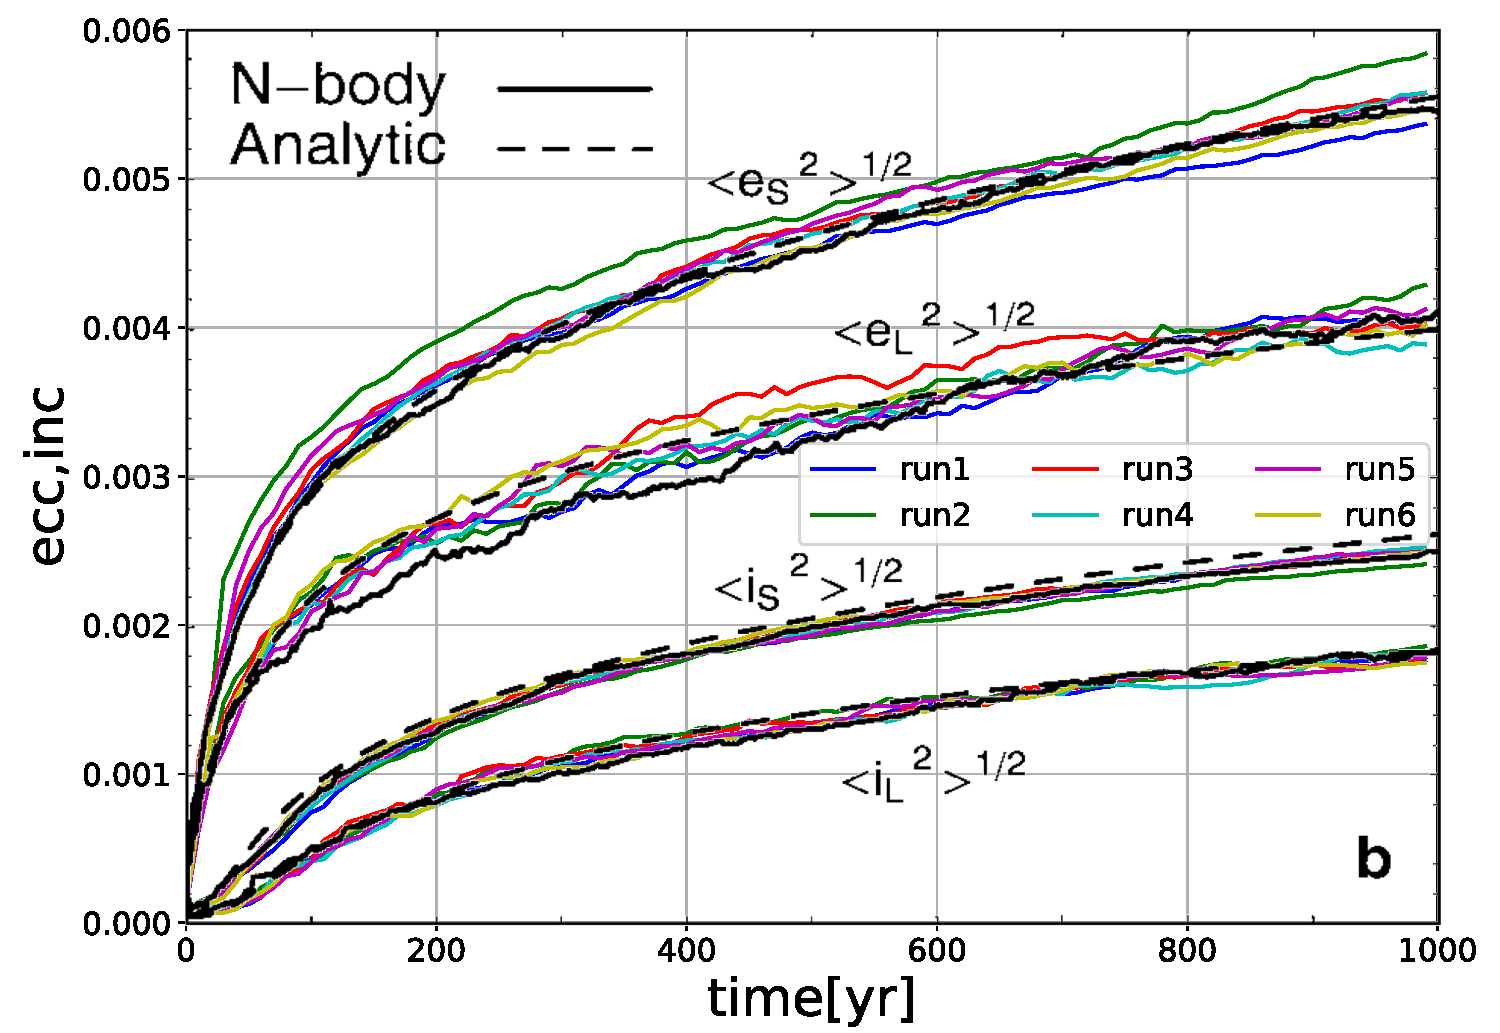
\includegraphics[width=8cm]{Ohtsuki_figb_and_Nbodytest_6run.pdf}
 %\caption{小さい微惑星と大きい微惑星が混在するときの離心率と軌道傾斜角の二乗平均平方根の時間進化。計算結果に\cite{Ohtsuki2002}のFig.4bを重ねたところ、よく再現できている。\label{fig:Nbody}}
%\end{figure}

%\subsection{統計的手法のテスト}
%統計的手法のテストとして\cite{Kobayashi2010}の解析解との比較を行った(図\ref{fig:Frag})。
%$0.95 - 1.05 {\rm AU}$に等質量のトレーサーを$990$個一様に配置し、トレーサー同士の重力相互作用は解かずに$10^4$年分計算を行った。初期の離心率と軌道傾斜角は$e = 10^{-3}, i = 5 \times 10^{-4}$であり、他の軌道要素は等間隔で与えた。質量減少タイムスケール$\tau_{\rm dep}=10$年となるように、初期の総質量$M_{\rm tot,0} = 3.51 \times 10^{30} {\rm g}$で与えた。$\delta r = 0.01 {\rm AU}, \delta \theta = \pi$で固定している。

%\begin{figure}[h]
 %\centering
 %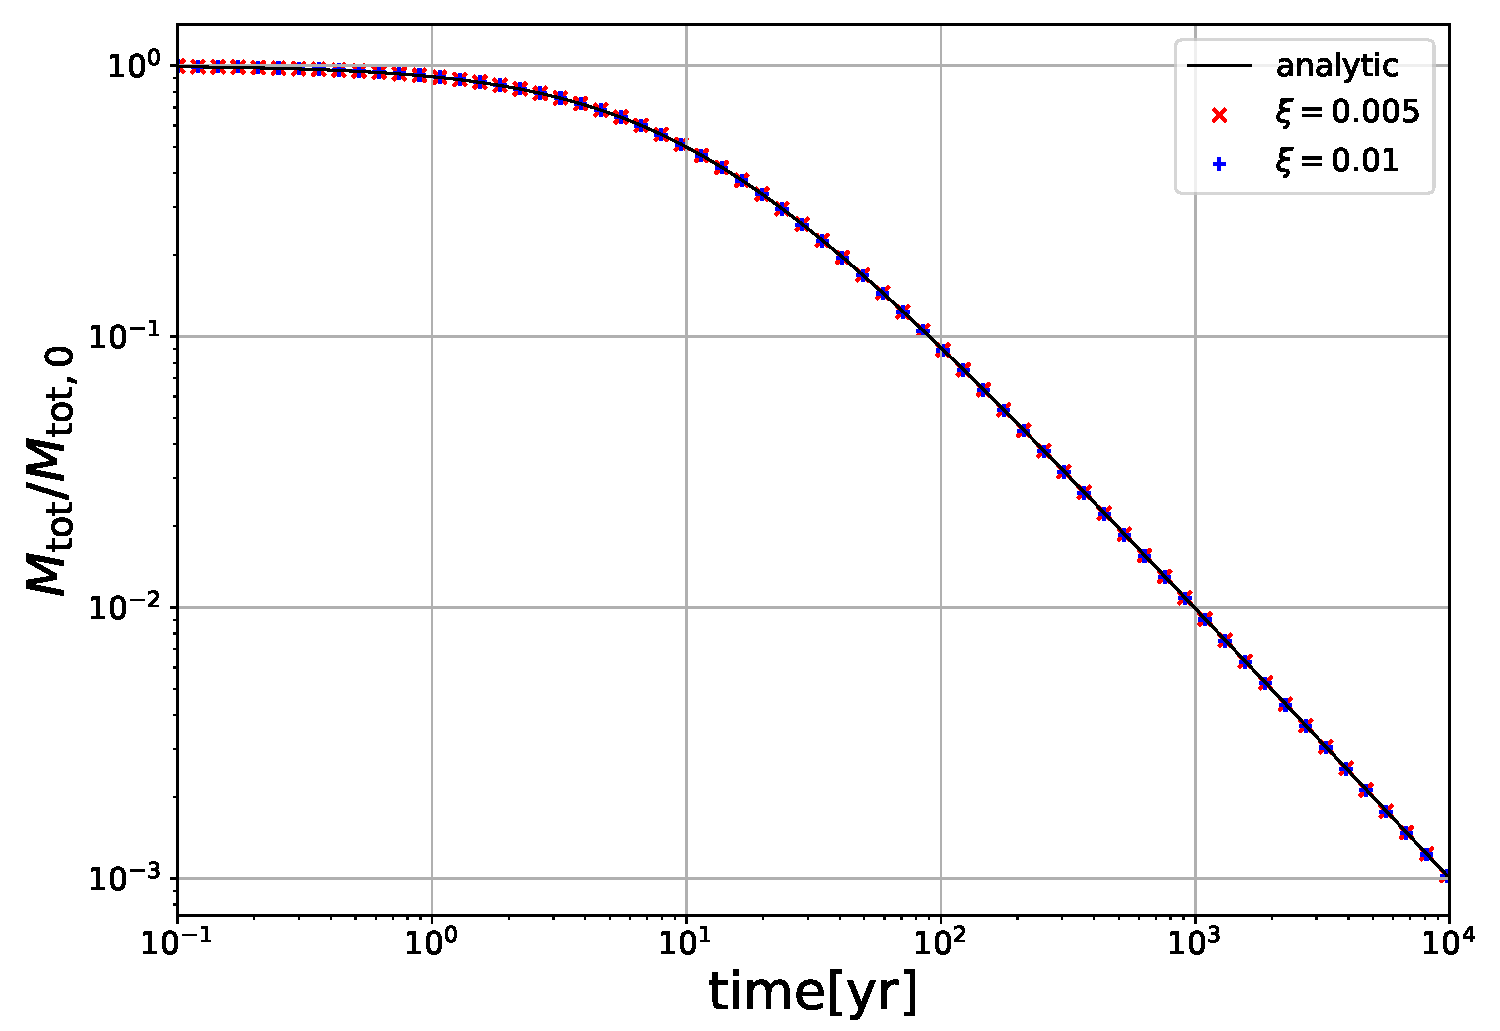
\includegraphics[width=8cm]{MassDepletion.pdf}
 %\caption{微惑星円盤の総質量の時間進化。解析解とほとんど一致している。\label{fig:Frag}}
%\end{figure}

\section{結果と考察}
地球型惑星と原始惑星の巨大衝突破壊によって破片が放出される様子を模擬し、惑星と破片の軌道進化と破片の質量進化を計算した。初期の破片の総質量は$0.1 {\rm M_{\oplus}}$とし、惑星の質量は$1 {\rm M_{\oplus}}$とした。$(x,y) = (1 {\rm AU},0 {\rm AU})$の位置で衝突が起こり、惑星から見て中心星と反対方向(L2側)に惑星表面からコーン状に破片が放出し、その速度は惑星から距離が離れるにつれて速くなると仮定した(脱出速度$v_{\rm esc}$の$1.0-1.1$倍)。破片を等質量のトレーサー1000個で代表させ、中心星周りのケプラー運動、惑星とトレーサーの重力相互作用、トレーサー同士の衝突破壊を、ハイブリッドコードを用いて1000年分計算を行った(図\ref{fig:L2cone})。円盤の内側にいくほど、相対速度は速くなり、また面密度が大きくなるため、トレーサー内の破片が衝突破壊によって減少し質量が減っている様子を見ることができる。
衝突カスケードにおいて破片のサイズ分布が$n(D) \propto D^{-7/2}$のとき、fractional luminosity(中心星とデブリ円盤の光度比)は
\begin{align}
 f = 0.37 \left(\frac{M_{\rm tot}}{\rm M_{\oplus}}\right) \left(\frac{r}{\rm AU}\right)^{-2} \left(\frac{D_{\rm min}}{\rm \mu m}\right)^{-\frac{1}{2}} \left(\frac{D_{\rm max}}{\rm km}\right)^{-\frac{1}{2}}
\end{align}
で表される\citep{Jackson2012}。これより、円盤の質量と光度は比例関係にあり、図\ref{fig:L2cone}の質量分布を明るさの空間分布として見ることもできる。

今後はこのハイブリッドコードを用いて、複数の原始惑星が存在し、巨大衝突が起こるたびに破片を放出するような計算を長時間行うことで、暖かいデブリ円盤の進化について詳しく調べたい。


%\begin{figure}[h]
% \centering
% 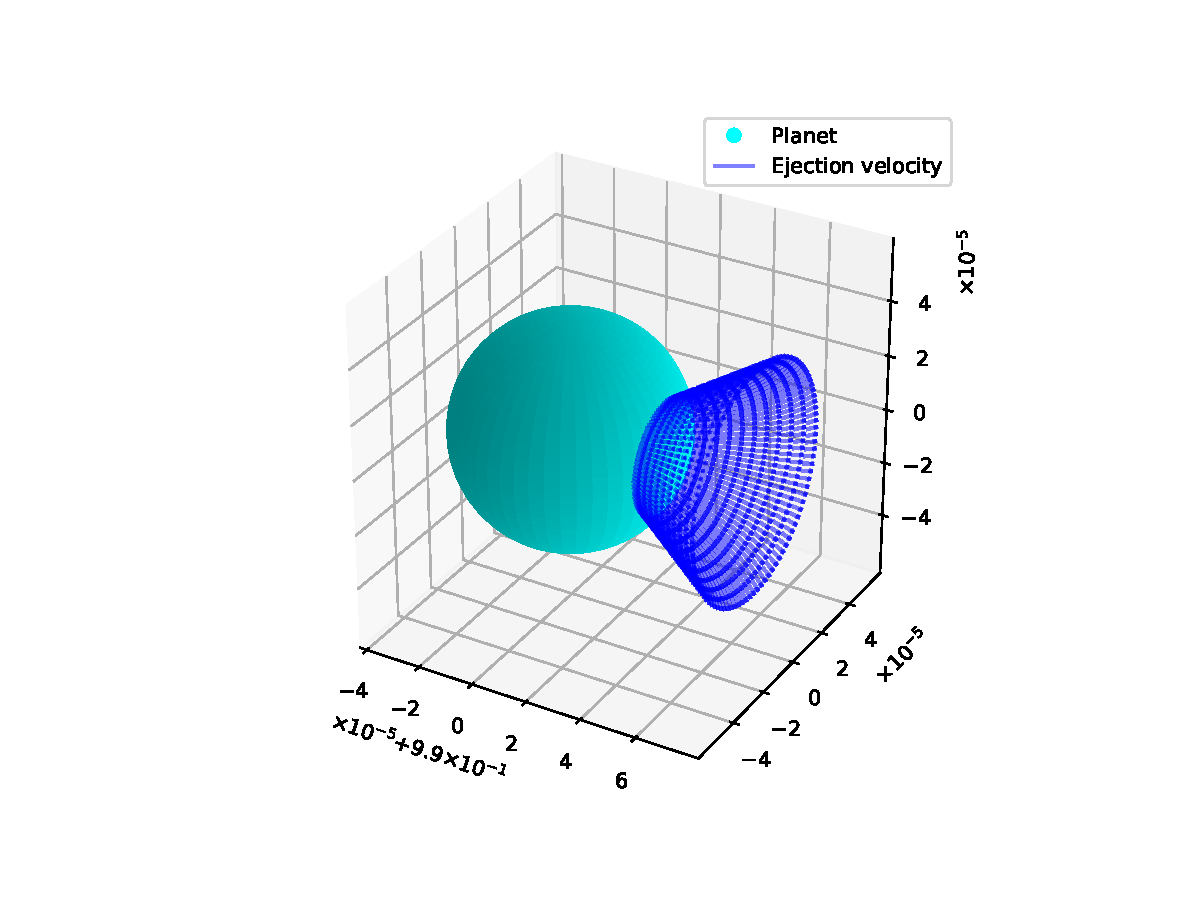
\includegraphics[width=5cm]{Ejection_cone30equidistant_v1011curl_3D.pdf}
% \caption{惑星半径$R_{\rm p} = 4 \times 10^{-5} {\rm AU}$の$1.0-2.0$倍の距離に角度$30^{\circ}$のコーンに沿って等間隔にトレーサーを置き、速度は脱出
%速度$v_{\rm esc}$の$1.0-1.1$倍で与えた。\label{fig:cone3D}}
%\end{figure}

\begin{figure}[h]
 \centering
 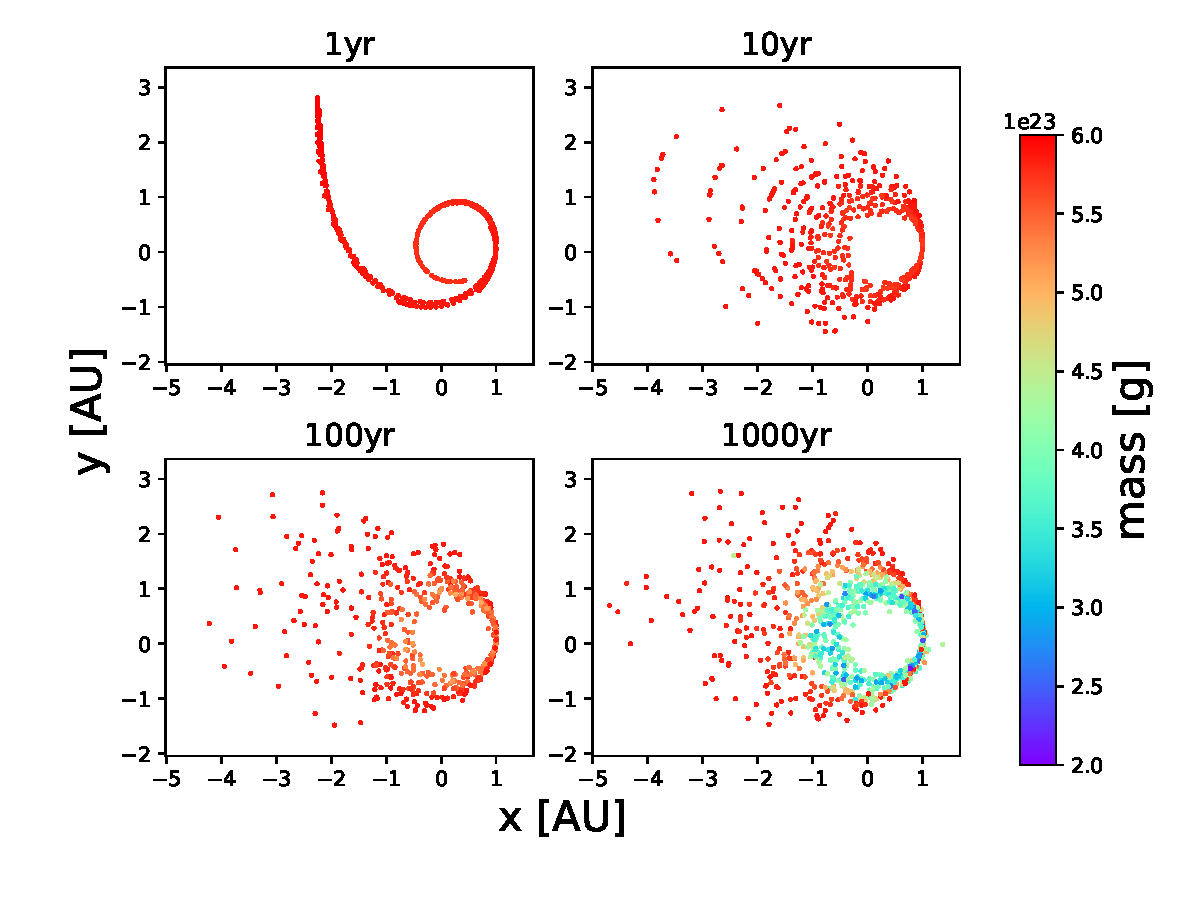
\includegraphics[width=8cm]{L2cone30equidistant_v1011curl_OnlyPlanet_1000yr.pdf}
 \caption{破片の軌道と質量の時間変化。トレーサーの位置を$x,y$平面に射影し、各点の色で質量を表した。
 %すべてのトレーサーの初期質量は${10^{-4}\rm M_{\oplus}}$である。
 破壊計算では$\delta r = 0.01 {\rm AU}, \delta \theta = \pi/2$で固定した。\label{fig:L2cone}}
\end{figure}









\section*{謝辞}
本研究を行うにあたり、様々なご指導を頂きました小林浩氏に深く感謝いたします。

\small
\begin{thebibliography}{99}
 \bibitem[Aarseth(1985)]{Aarseth1985}
 Aarseth, S. J. 1985, in Multiple Time Scales, ed. J. U. Brackbill and B. I. Cohen (New York:Academic), 377
 \bibitem[Genda et al.(2015)]{Genda2015}
 Genda, H., Kobayashi, H., \& Kokubo, E. 2015, ApJ, 810, 136 
 \bibitem[Genda et al.(2012)]{Genda2012}
 Genda, H., Kokubo, E., \& Ida, S. 2012, ApJ, 744, 137
 \bibitem[Jackson \& Wyatt(2012)]{Jackson2012}
 Jackson, A. P. \& Wyatt, M. C. 2012, MNRAS, 425, 657
 \bibitem[Kobayashi \& Tanaka(2010)]{Kobayashi2010}
 Kobayashi, H., \& Tanaka, H. 2010, Icarus, 206, 735
 \bibitem[Lisse et al.(2008)]{Lisse2008}
 Lisse, C. M., Chen, C. H., Wyatt, M. C. \& Morlok, A. 2008, ApJ, 673, 1106
 \bibitem[Lisse et al.(2009)]{Lisse2009}
 Lisse, C. M., Chen, C. H., Wyatt, M. C., Morlok, A., Song, I., Bryden, G. \& Sheeham, P. 2009, ApJ, 791, 2019
 \bibitem[Makino(1991)]{Makino1991}
 Makino, J. 1991, ApJ, 369, 200
 \bibitem[Makino \& Aarseth(1992)]{Makino1992}
 Makino, J., \& Aarseth, S. J. 1992, PASJ, 44, 141
 \bibitem[Morishima(2015)]{Morishima2015}
 Morishima, R. 2015, Icarus, 260, 368
 \bibitem[Ohtsuki et al.(2002)]{Ohtsuki2002}
 Ohtsuki, K., Stewart, G. R., \& Ida, S. 2002, Icarus, 155, 436
 \bibitem[Tanaka et al.(1996)]{Tanaka1996}
 Tanaka, H., Inaba, S., Nakazawa, K. 1996, Icarus, 123, 450
 
\end{thebibliography}






\end{document}